\section{Связность в орграфе}
Определить для орграфа заданного матрицей смежности:

$A = \begin{pmatrix}
0 & 1 & 1 & 0\\
0 & 0 & 1 & 1\\
1 & 0 & 0 & 0\\
1 & 1 & 1 & 0
\end{pmatrix}$

\begin{enumerate}
\item[а)] Матрицу односторонней связности;
\item[б)] Матрицу сильной связности
\item[в)] Компоненты сильной связности;
\item[г)] Матрицу контуров.
\end{enumerate}
\subsection{Матрица односторонней связности}
\begin{enumerate}
    \item [1)] $A^2 = \begin{pmatrix}
0 & 1 & 1 & 0\\
0 & 0 & 1 & 1\\
1 & 0 & 0 & 0\\
1 & 1 & 1 & 0
\end{pmatrix}\begin{pmatrix}
0 & 1 & 1 & 0\\
0 & 0 & 1 & 1\\
1 & 0 & 0 & 0\\
1 & 1 & 1 & 0
\end{pmatrix} = \begin{pmatrix}
1 & 0 & 1 & 1\\
1 & 1 & 1 & 0\\
0 & 1 & 1 & 0\\
1 & 1 & 1 & 1
\end{pmatrix}$.
    \item[2)] $A^3 = \begin{pmatrix}
1 & 0 & 1 & 1\\
1 & 1 & 1 & 0\\
0 & 1 & 1 & 0\\
1 & 1 & 1 & 1
\end{pmatrix}\begin{pmatrix}
0 & 1 & 1 & 0\\
0 & 0 & 1 & 1\\
1 & 0 & 0 & 0\\
1 & 1 & 1 & 0
\end{pmatrix} = \begin{pmatrix}
1 & 1 & 1 & 0\\
1 & 1 & 1 & 1\\
1 & 0 & 1 & 1\\
1 & 1 & 1 & 1
\end{pmatrix}$.
    \item[3)] $T = E \lor A \lor A^2 \lor A^3 = \begin{pmatrix}
1 & 0 & 0 & 0\\
0 & 1 & 0 & 0\\
0 & 0 & 1 & 0\\
0 & 0 & 0 & 1
\end{pmatrix}\lor\begin{pmatrix}
0 & 1 & 1 & 0\\
0 & 0 & 1 & 1\\
1 & 0 & 0 & 0\\
1 & 1 & 1 & 0
\end{pmatrix}\lor\begin{pmatrix}
1 & 0 & 1 & 1\\
1 & 1 & 1 & 0\\
0 & 1 & 1 & 0\\
1 & 1 & 1 & 1
\end{pmatrix}\lor\begin{pmatrix}
1 & 1 & 1 & 0\\
1 & 1 & 1 & 1\\
1 & 0 & 1 & 1\\
1 & 1 & 1 & 1
\end{pmatrix} = \begin{pmatrix}
1 & 1 & 1 & 1\\
1 & 1 & 1 & 1\\
1 & 1 & 1 & 1\\
1 & 1 & 1 & 1
\end{pmatrix}$ = $T$ - матрица односторонней связности
\end{enumerate}
\begin{center}
    Найдем матрицу односторонней связности по итерационному алгоритму Уоршалла.
\end{center}
\begin{enumerate}
    \item[] \begin{center}
        $k = 0$
            \end{center}
        $T^{(0)} = E \lor A = \begin{pmatrix}
1 & 0 & 0 & 0\\
0 & 1 & 0 & 0\\
0 & 0 & 1 & 0\\
0 & 0 & 0 & 1
\end{pmatrix}\lor\begin{pmatrix}
0 & 1 & 1 & 0\\
0 & 0 & 1 & 1\\
1 & 0 & 0 & 0\\
1 & 1 & 1 & 0
\end{pmatrix} = \begin{pmatrix}
1 & 1 & 1 & 0\\
0 & 1 & 1 & 1\\
1 & 0 & 1 & 0\\
1 & 1 & 1 & 1
\end{pmatrix}$
    \item[] \begin{center}
        $k = 1,  k - 1 = 0$
            \end{center}
        $T^{(1)} = \begin{pmatrix}
1 & 1 & 1 & 0\\
0 & 1 & 1 & 1\\
1 & 0 & 1 & 0\\
1 & 1 & 1 & 1
\end{pmatrix}\lor\begin{pmatrix}
0 & 0 & 0 & 0\\
0 & 0 & 0 & 0\\
0 & 1 & 1 & 0\\
0 & 1 & 1 & 0
\end{pmatrix} = \begin{pmatrix}
1 & 1 & 1 & 0\\
0 & 1 & 1 & 1\\
1 & 1 & 1 & 0\\
1 & 1 & 1 & 1
\end{pmatrix}$
    \item[] \begin{center}
        $k = 2,  k - 1 = 1$
            \end{center}
        $T^{(2)} = \begin{pmatrix}
1 & 1 & 1 & 0\\
0 & 1 & 1 & 1\\
1 & 1 & 1 & 0\\
1 & 1 & 1 & 1
\end{pmatrix}\lor\begin{pmatrix}
0 & 1 & 1 & 1\\
0 & 1 & 1 & 1\\
0 & 1 & 1 & 1\\
0 & 1 & 1 & 1
\end{pmatrix} = \begin{pmatrix}
1 & 1 & 1 & 1\\
0 & 1 & 1 & 1\\
1 & 1 & 1 & 1\\
1 & 1 & 1 & 1
\end{pmatrix}$
\item[] \begin{center}
        $k = 3,  k - 1 = 2$
            \end{center}
        $T^{(3)} = \begin{pmatrix}
1 & 1 & 1 & 1\\
0 & 1 & 1 & 1\\
1 & 1 & 1 & 1\\
1 & 1 & 1 & 1
\end{pmatrix}\lor\begin{pmatrix}
1 & 1 & 1 & 1\\
1 & 1 & 1 & 1\\
1 & 1 & 1 & 1\\
1 & 1 & 1 & 1
\end{pmatrix} = \begin{pmatrix}
1 & 1 & 1 & 1\\
1 & 1 & 1 & 1\\
1 & 1 & 1 & 1\\
1 & 1 & 1 & 1
\end{pmatrix}$
\item[] \begin{center}
        $k = 4,  k - 1 = 3$
            \end{center}
        $T^{(4)} = \begin{pmatrix}
1 & 1 & 1 & 1\\
1 & 1 & 1 & 1\\
1 & 1 & 1 & 1\\
1 & 1 & 1 & 1
\end{pmatrix}\lor\begin{pmatrix}
1 & 1 & 1 & 1\\
1 & 1 & 1 & 1\\
1 & 1 & 1 & 1\\
1 & 1 & 1 & 1
\end{pmatrix} = \begin{pmatrix}
1 & 1 & 1 & 1\\
1 & 1 & 1 & 1\\
1 & 1 & 1 & 1\\
1 & 1 & 1 & 1
\end{pmatrix} = T$.
\end{enumerate}
\subsection{Матрица сильной связности}

$\overset{-}{S} = T \& T^{T} = \begin{pmatrix}
1 & 1 & 1 & 1\\
1 & 1 & 1 & 1\\
1 & 1 & 1 & 1\\
1 & 1 & 1 & 1
\end{pmatrix}\lor\begin{pmatrix}
1 & 1 & 1 & 1\\
1 & 1 & 1 & 1\\
1 & 1 & 1 & 1\\
1 & 1 & 1 & 1
\end{pmatrix} = \begin{pmatrix}
1 & 1 & 1 & 1\\
1 & 1 & 1 & 1\\
1 & 1 & 1 & 1\\
1 & 1 & 1 & 1
\end{pmatrix}$
\subsection{Компоненты сильной связности}
Одна компонента сильной связности: $\{v_1, v_2, v_3, v_4\}$
\subsection{Матрица контуров}
$K = \overset{-}{S}\&A = \begin{pmatrix}
1 & 1 & 1 & 1\\
1 & 1 & 1 & 1\\
1 & 1 & 1 & 1\\
1 & 1 & 1 & 1
\end{pmatrix}\&\begin{pmatrix}
0 & 1 & 1 & 0\\
0 & 0 & 1 & 1\\
1 & 0 & 0 & 0\\
1 & 1 & 1 & 0
\end{pmatrix} = \begin{pmatrix}
0 & 1 & 1 & 0\\
0 & 0 & 1 & 1\\
1 & 0 & 0 & 0\\
1 & 1 & 1 & 0
\end{pmatrix}$
\newpage
\section{Алгоритм Тэрри}
\begin{figure}[!htb]
	\centering
	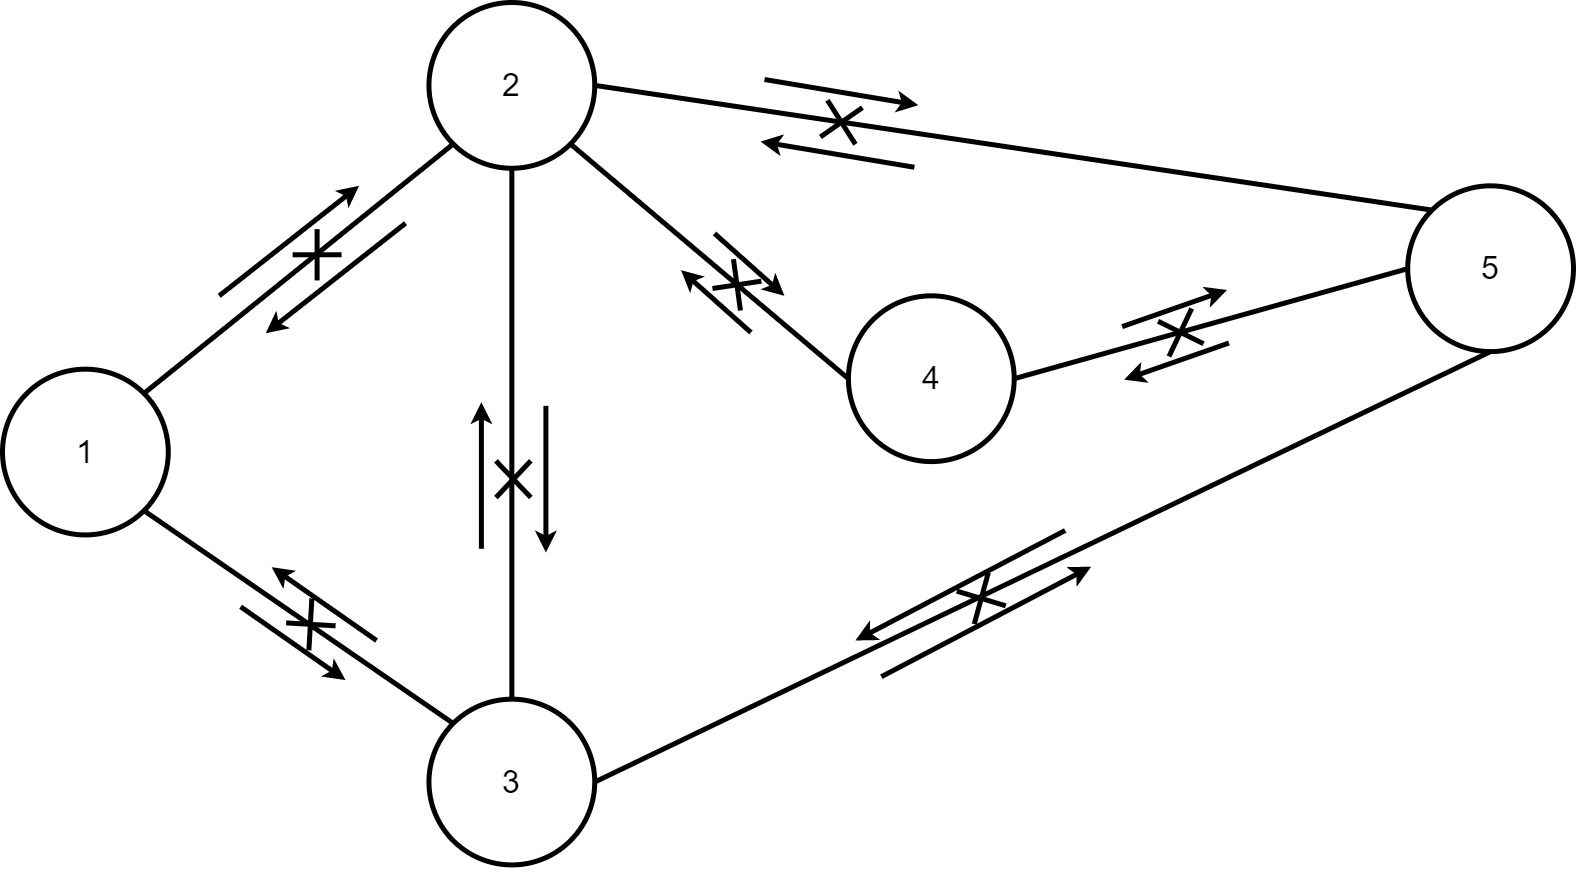
\includegraphics[width=\textwidth]{Images/graph1.jpg}
	\caption{Граф}
	\label{fig:image1}
\end{figure}
\textbf{Маршрут обхода}:
1 - 2 - 3 - 5 - 4 - 2 - 5 - 3 - 1 - 3 - 2 - 4 - 5 - 2 - 1
\newpage
\section{Алгоритм "фронта волны"}

$A = \begin{pmatrix}
0 & 0 & 0 & 1 & 0 & 0 & 1 & 0\\
1 & 0 & 1 & 1 & 0 & 1 & 0 & 1\\
1 & 1 & 0 & 1 & 1 & 1 & 0 & 0\\
0 & 0 & 1 & 0 & 1 & 1 & 1 & 0\\
1 & 1 & 1 & 1 & 0 & 1 & 1 & 0\\
1 & 1 & 1 & 0 & 1 & 0 & 0 & 0\\
0 & 0 & 1 & 0 & 1 & 1 & 0 & 0\\
0 & 1 & 1 & 1 & 0 & 0 & 1 & 0\\
\end{pmatrix}$

\begin{enumerate}
    \item[]$W_0 = v_1$
    \item[]$\Gamma W_0(v_1) = \{v_4, v_7 \} =
W_1(v_1)
$
    \item[]$\Gamma W_1(v_1)\backslash\{W_0 \cap W_1\} = \{v_3, v_5, v_6 \} =
W_2(v_1)
$
\item[]$\Gamma W_2(v_1)\backslash\{W_0 \cap W_1 \cap W_2\} = \{v_2\} =
W_3(v_1)
$
\item[]$\Gamma W_3(v_1)\backslash\{W_0 \cap W_1 \cap W_2 \cap W_3\} = \{v_8\} =
W_4(v_1)
$
\end{enumerate}
\begin{enumerate}
    \item[] $W_4 = v_8$
    \item[] $W_3 = W_3(v_1) \cap \Gamma^{-1}(W_4) = \{ v_2 \}$
    \item[] $W_2 = W_2(v_1) \cap \Gamma^{-1}(W_3) = \{ v_3, v_5, v_6 \}$
    \item[] $W_1 = W_1(v_1) \cap \Gamma^{-1}(W_2) = \{ v_4, v_7\}$
    \item[] $W_0 = W_0(v_1) \cap \Gamma^{-1}(W_1) = \{ v_1\}$
\end{enumerate}
\newpage
Кратчайшие пути = 6:

$v_1 - v_4 - v_3 - v_2 - v_8$

$v_1 - v_4 - v_5 - v_2 - v_8$

$v_1 - v_4 - v_6 - v_2 - v_8$

$v_1 - v_7 - v_3 - v_2 - v_8$

$v_1 - v_7 - v_5 - v_2 - v_8$

$v_1 - v_7 - v_6 - v_2 - v_8$
\begin{figure}[!htb]
	\centering
	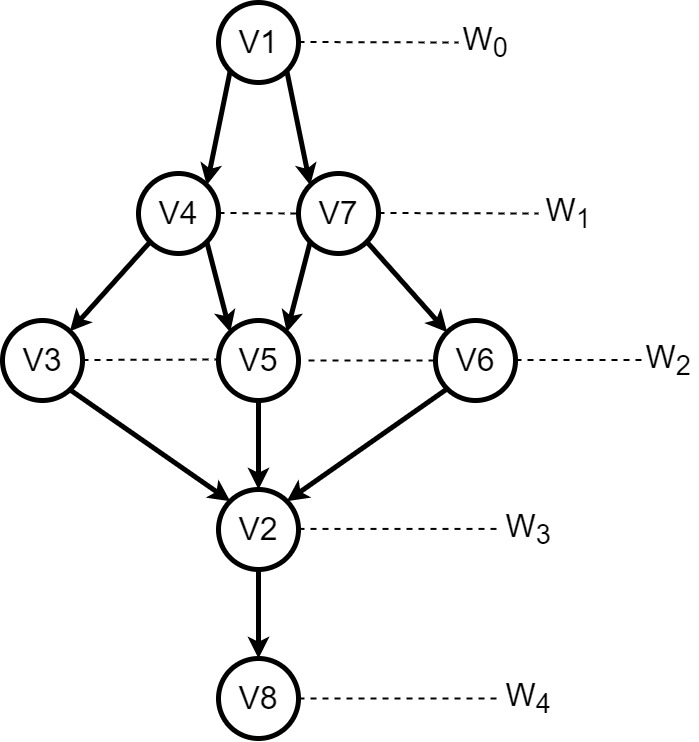
\includegraphics[width=\textwidth]{Images/graph2.jpg}
	\caption{Алгоритм Фронта волны}
	\label{fig:image2}
\end{figure}
\newpage
\section{Алгоритм Форда}
$C = \begin{pmatrix}
\infty & 4 & 5 & 3 & \infty & \infty &
\infty\\
10 & \infty & 2 & \infty & 3 & \infty &
\infty\\
\infty & 2 & \infty & 3 & 1 & 4 & 7\\
\infty & \infty & 2 & \infty & \infty & 7
& \infty\\
\infty & \infty & 1 & \infty & \infty &
\infty & 4\\
\infty & \infty & 4 & \infty & \infty &
\infty & 2\\
2 & \infty & 3 & \infty & 5 & 7 & \infty\\
\end{pmatrix}$
\begin{figure}[!htb]
	\centering
	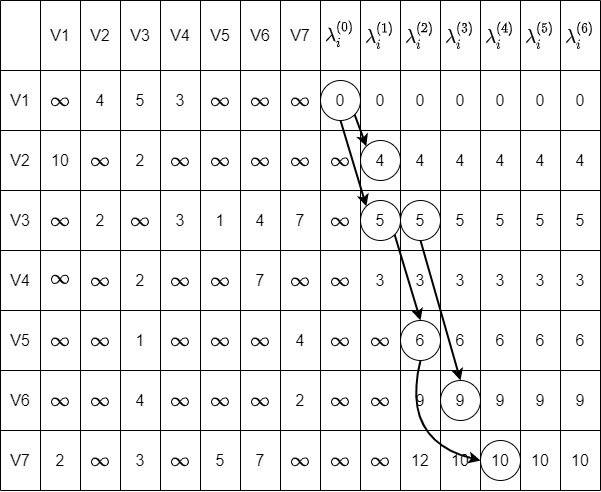
\includegraphics[width=\textwidth]{Images/graph3.jpg}
	\caption{Алгоритм Форда}
	\label{fig:image3}
\end{figure}
\newpage
\begin{enumerate}
    \item Минимальный путь из $v1$ в $v2$:
    
    $v1 - v2$
    
    $\lambda^{(0)}_1 + C_{12} = 0 + 4 = \lambda^{(1)}_2$
     \item Минимальный путь из $v1$ в $v3$:
    
    $v1 - v3$
    
    $\lambda^{(0)}_1 + C_{13} = 0 + 5 = \lambda^{(1)}_3$
     \item Минимальный путь из $v1$ в $v4$:
    
    $v1 - v4$
    
    $\lambda^{(0)}_1 + C_{14} = 0 + 3 = \lambda^{(1)}_4$
     \item Минимальный путь из $v1$ в $v5$:
    
    $v1 - v3 - v5$
    
    $\lambda^{(0)}_1 + C_{13} = \lambda^{(1)}_3$
    
    $\lambda^{(1)}_3 + C_{35} = \lambda^{(2)}_5$
     \item Минимальный путь из $v1$ в $v6$:
    
    $v1 - v3 - v6$
    
    $\lambda^{(0)}_1 + C_{13} = \lambda^{(1)}_3$
    
    $\lambda^{(1)}_3 + C_{36} = \lambda^{(2)}_6$
     \item Минимальный путь из $v1$ в $v7$:
    
    $v1 - v3 - v5 - v7$
    
    $\lambda^{(0)}_1 + C_{13} = \lambda^{(1)}_3$
    
    $\lambda^{(1)}_3 + C_{35} = \lambda^{(2)}_5$
    
    $\lambda^{(2)}_5 + C_{57} = \lambda^{(3)}_7$
\end{enumerate}
\section{Остовое дерево минимальной длины}
\begin{figure}[!htb]
	\centering
	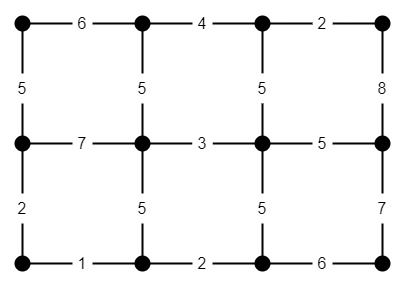
\includegraphics[width=\linewidth]{Images/graph4.jpg}
	\caption{Исходный граф}
	\label{fig:image4}
\end{figure}

\begin{figure}[H]
\begin{minipage}[h]{0.47\linewidth}
\center{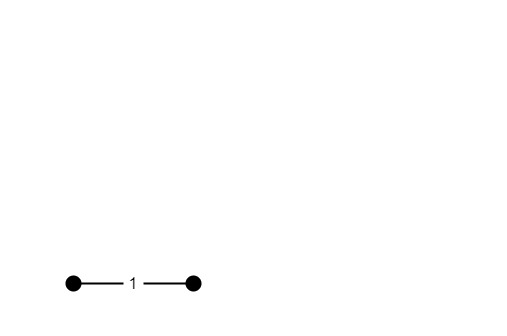
\includegraphics[width=1\linewidth]{Images/graph5.jpg}} 1) \\
\end{minipage}
\hfill
\begin{minipage}[h]{0.47\linewidth}
\center{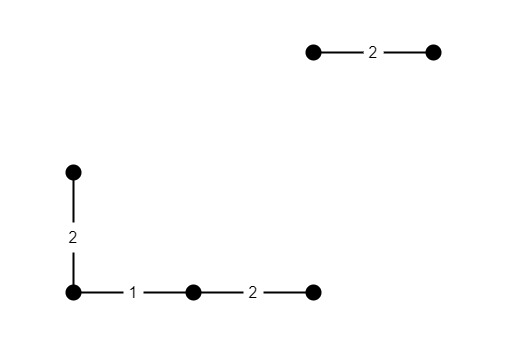
\includegraphics[width=1\linewidth]{Images/graph6.jpg}} \\2)
\end{minipage}
\vfill
\begin{minipage}[h]{0.47\linewidth}
\center{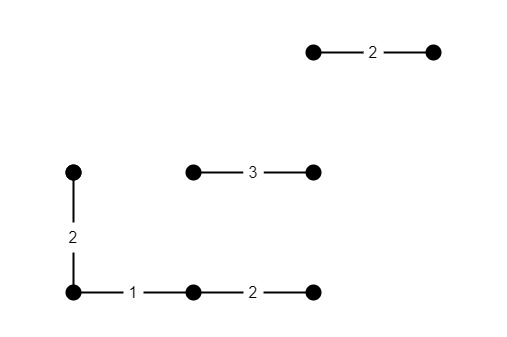
\includegraphics[width=1\linewidth]{Images/graph7.jpg}} 3) \\
\end{minipage}
\hfill
\begin{minipage}[h]{0.47\linewidth}
\center{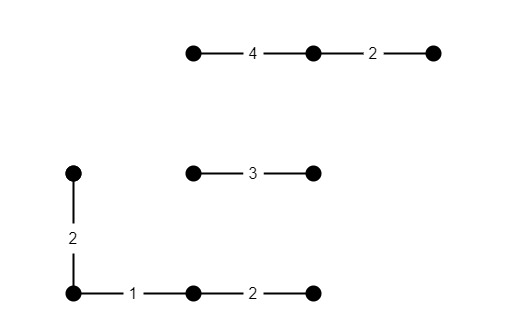
\includegraphics[width=1\linewidth]{Images/graph8.jpg}} 4) \\
\end{minipage}
\vfill
\begin{minipage}[h]{0.47\linewidth}
\center{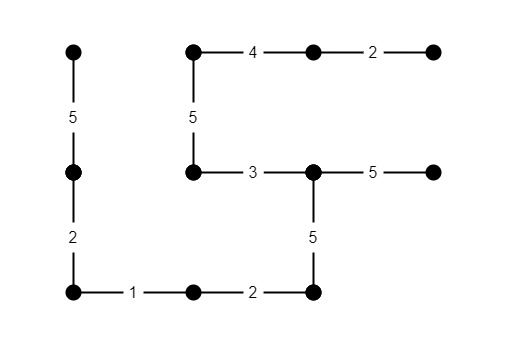
\includegraphics[width=1\linewidth]{Images/graph9.jpg}} 5) \\
\end{minipage}
\hfill
\begin{minipage}[h]{0.47\linewidth}
\center{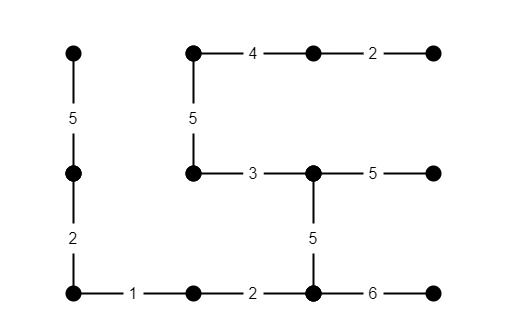
\includegraphics[width=1\linewidth]{Images/graph10.jpg}} 6) \\
\end{minipage}
\caption{Остовое дерево минимальной длины}
\label{ris:experimentalcorrelationsignals}
\end{figure}
Минимальный вес остового дерева $L(D) = 40$
\newpage
\section{Деревья и циклы}
\begin{enumerate}
    \item[] \begin{figure}[!htb]
	\centering
	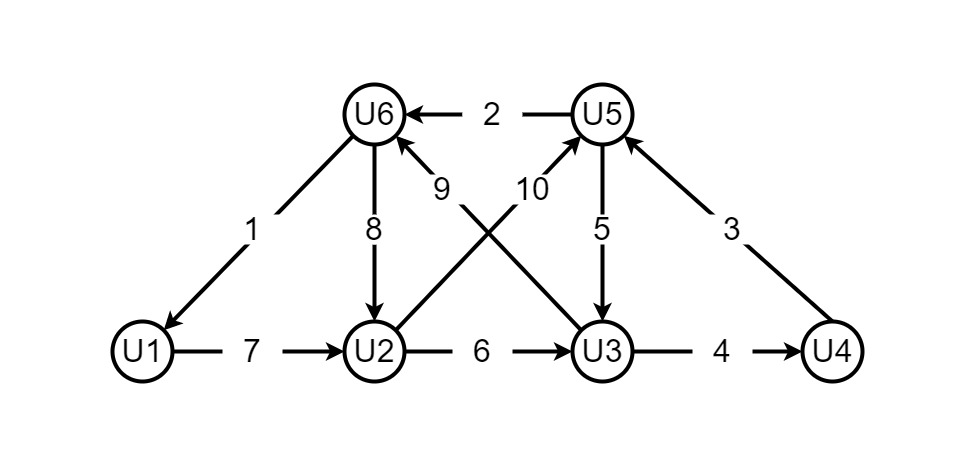
\includegraphics[width=\linewidth]{Images/graph11.jpg}
	\caption{1) Зададим произвольную ориентацию}
	\label{fig:image5}
	\end{figure}
    \item[] \begin{figure}[!htb]
	\centering
	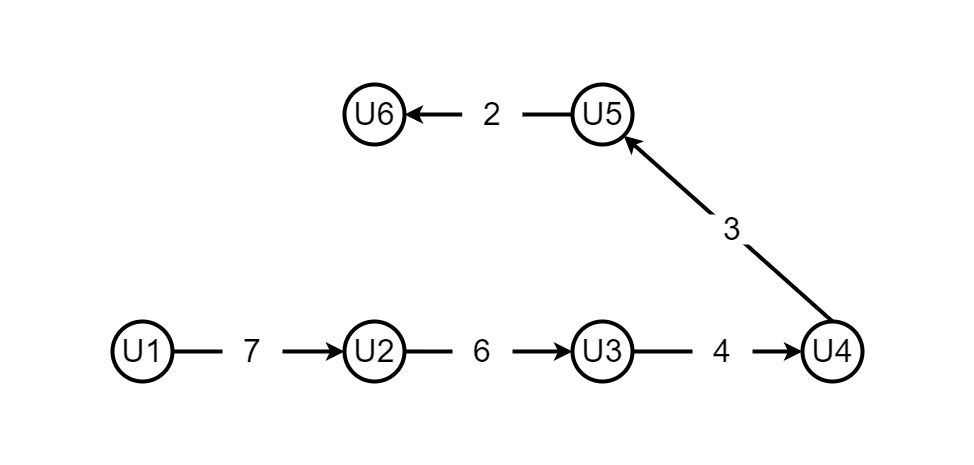
\includegraphics[width=\linewidth]{Images/graph12.jpg}
	\caption{2) Построим произвольное остовое дерево D заданного графа}
	\label{fig:image6}
	\end{figure}
	\newpage
	\item[3)] Найдем базис циклов, добавляя к остовному дереву по одному не вошедшему в него ребру. Затем найдем соответствующие вектор-циклы.
	
	$(D+q_1) \ \mu_1:\ v_1 \to v_2 \to v_3 \to v_4 \to v_5 \to v_6 \to v_1 \ \Rightarrow \ \\ c(\mu_1) = (1,1,1,1,0,1,1,0,0,0)$
	
	$(D+q_5) \ \mu_2:\ v_3 \to v_4 \to v_5 \to v_3 \ \Rightarrow \ \\ c(\mu_2) = (0,0,1,1,1,0,0,0,0,0)$
	
	$(D+q_9) \ \mu_3:\ v_3 \to v_4 \to v_5 \to v_6 \to v_3 \ \Rightarrow \ \\ c(\mu_3) = (0,1,1,1,0,0,0,0,-1,0)$
	
	$(D+q_{10}) \ \mu_4:\ v_2 \to v_3 \to v_4 \to v_5 \to v_2 \ \Rightarrow \ \\ c(\mu_4) = (0,0,1,1,0,1,0,0,0,-1)$
	
	$(D+q_{8}) \ \mu_5:\ v_2 \to v_3 \to v_4 \to v_5 \to v_6 \to v_2 \ \Rightarrow \ \\ c(\mu_5) = (0,1,1,1,0,1,0,1,0,0)$
	\item[4)] Цикломатическая матрица графа имеет вид: \\
    С = $\begin{pmatrix}
1 & 1 & 1 & 1 & 0 & 1 & 1 & 0 & 0 & 0\\
1 & 1 & 1 & 1 & 0 & 1 & 1 & 0 & 0 & 0\\
1 & 1 & 1 & 1 & 0 & 1 & 1 & 0 & 0 & 0\\
1 & 1 & 1 & 1 & 0 & 1 & 1 & 0 & 0 & 0\\
1 & 1 & 1 & 1 & 0 & 1 & 1 & 0 & 0 & 0\\
\end{pmatrix}$
    \newpage
    \item[5)] Выпишем закон Кирхгова для напряжений:\\
    $\begin{pmatrix}
1 & 1 & 1 & 1 & 0 & 1 & 1 & 0 & 0 & 0\\
1 & 1 & 1 & 1 & 0 & 1 & 1 & 0 & 0 & 0\\
1 & 1 & 1 & 1 & 0 & 1 & 1 & 0 & 0 & 0\\
1 & 1 & 1 & 1 & 0 & 1 & 1 & 0 & 0 & 0\\
1 & 1 & 1 & 1 & 0 & 1 & 1 & 0 & 0 & 0\\
\end{pmatrix}\begin{pmatrix}
u_1\\
u_2\\
u_3\\
u_4\\
u_5\\
u_6\\
u_7\\
u_8\\
u_9\\
u_{10}\\
\end{pmatrix} = 0$ \\
Напряжения, соответствующие ребрам, не вошедшим в остовное дерево – базисные переменные системы. \\
$\begin{cases}
u_1 + u_2 + u_3 + u_4 + u_6 + u_7 = 0 \\
u_3 + u_4 + u_5 = 0 \\
u_2 + u_3 + u_4 - u_9 = 0 \\
u_3 + u_4 + u_6 - u_{10} = 0 \\
u_2 + u_3 + u_4 + u_6 + u_8 = 0
\end{cases}
\Rightarrow
\begin{cases}
u_1 = -u_2 - u_3 - u_4 - u_6 - u_7 \\
u_5 = -u_3 - u_4 \\
u_9 = u_2 + u_3 + u_4 \\
u_{10} = u_3 + u_4 + u_6 \\
u_8 = -u_2 - u_3 - u_4 - u_6
\end{cases}$
\item[6)] Выпишем закон Кирхгова для токов:  \\
\textbf{\[B\cdot I = 0\]}
\newpage
\item[7)] Выпишем уравнения Кирхгофа для токов.\\
Найдем матрицу инцендентности $B$ орграфа: \\
$B = \begin{pmatrix}
1 & 0 & 0 & 0 & 0 & 0 & -1 & 0 & 0 & 0\\
0 & 0 & 0 & 0 & 0 & -1 & 1 & 1 & 0 & -1\\
0 & 0 & 0 & -1 & 1 & 1 & 0 & 0 & -1 & 0\\
0 & 0 & -1 & 1 & 0 & 0 & 0 & 0 & 0 & 0\\
0 & -1 & 1 & 0 & -1 & 0 & 0 & 0 & 0 & 1\\
-1 & 1 & 1 & 0 & -1 & 0 & 0 & -1 & 1 & 1
\end{pmatrix}$\\
$B \cdot I = \begin{pmatrix}
1 & 0 & 0 & 0 & 0 & 0 & -1 & 0 & 0 & 0\\
0 & 0 & 0 & 0 & 0 & -1 & 1 & 1 & 0 & -1\\
0 & 0 & 0 & -1 & 1 & 1 & 0 & 0 & -1 & 0\\
0 & 0 & -1 & 1 & 0 & 0 & 0 & 0 & 0 & 0\\
0 & -1 & 1 & 0 & -1 & 0 & 0 & 0 & 0 & 1\\
-1 & 1 & 1 & 0 & -1 & 0 & 0 & -1 & 1 & 1
\end{pmatrix}\begin{pmatrix}
I_1\\
I_2\\
I_3\\
I_4\\
I_5\\
I_6\\
I_7\\
I_8\\
I_9\\
I_{10}\\
\end{pmatrix} = 0
$ \\
$\begin{cases}
I_1 - I_7 = 0 \\
-I_6 + I_7 + I_8 - I_10 = 0 \\
-I_4 + I_5 + I_6 - I_9 = 0 \\
-I_3 + I_4 = 0 \\
-I_2 + I_3 - I_5 + I_{10} = 0 \\
-I_1 + I_2 - I_8 + I_9 = 0
\end{cases}
\Rightarrow
\begin{cases}
I_1 - I_7 = 0 \\
-I_6 + I_7 + I_8 - I_10 = 0 \\
-I_4 + I_5 + I_6 - I_9 = 0 \\
-I_3 + I_4 = 0 \\
-I_2 + I_3 - I_5 + I_{10} = 0
\end{cases}$
\newpage
\item[8)] Подставим закон Ома:\\
$\begin{cases}
E_1 = -I_2R_2 - I_3R_3 - I_4R_4 - I_6R_6 - I_7R_7 \\
E_2 = -I_3R_3 - I_4R_4 \\
0 = I_2R_2 + I_3R_3 + I_4R_4 - I_9R_9\\
0 = I_3R_3 + I_4R_4 + I_6R_6 - I_{10}R_{10}\\
0 = I_2R_2 + I_3R_3 + I_4R_4 + I_6R_6 + I_8R_8
\end{cases}$
\item[9)] Совместная система имеет вид: \\
$\begin{cases}
I_1 - I_7 = 0 \\
-I_6 + I_7 + I_8 - I_10 = 0 \\
-I_4 + I_5 + I_6 - I_9 = 0 \\
-I_3 + I_4 = 0 \\
-I_2 + I_3 - I_5 + I_{10} = 0 \\
E_1 = -I_2R_2 - I_3R_3 - I_4R_4 - I_6R_6 - I_7R_7 \\
E_2 = -I_3R_3 - I_4R_4 \\
0 = I_2R_2 + I_3R_3 + I_4R_4 - I_9R_9\\
0 = I_3R_3 + I_4R_4 + I_6R_6 - I_{10}R_{10}\\
0 = I_2R_2 + I_3R_3 + I_4R_4 + I_6R_6 + I_8R_8
\end{cases}$
\end{enumerate}
\newpage
\section{Транспортные сети}
\begin{figure}[!htb]
\centering
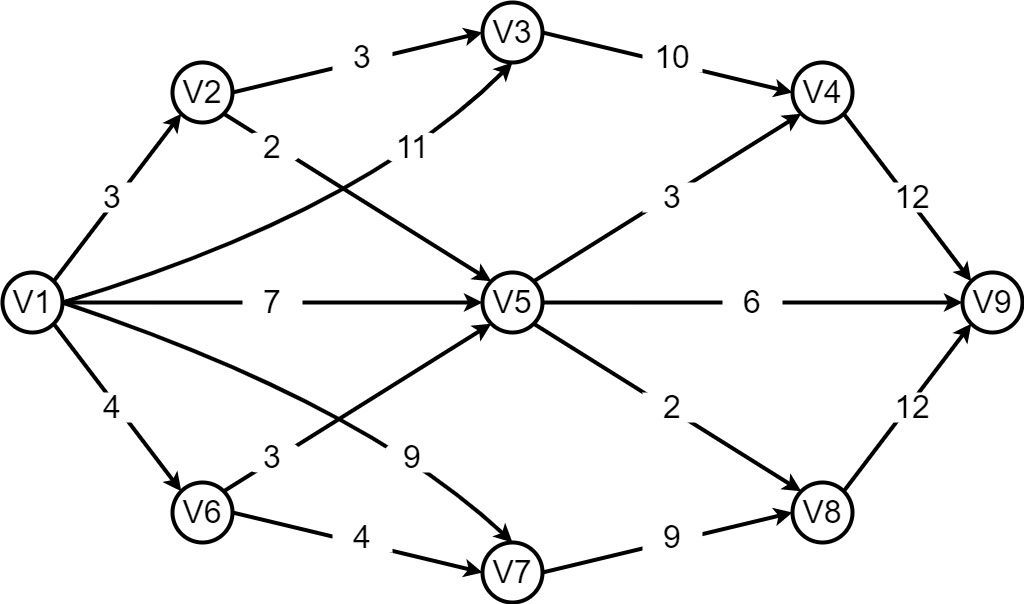
\includegraphics[width=\linewidth]{Images/graph13.jpg}
\caption{Транспортные сети}
\label{fig:image7}
\end{figure}
\subsection{Построение полного потока}
\begin{figure}[!htb]
\centering
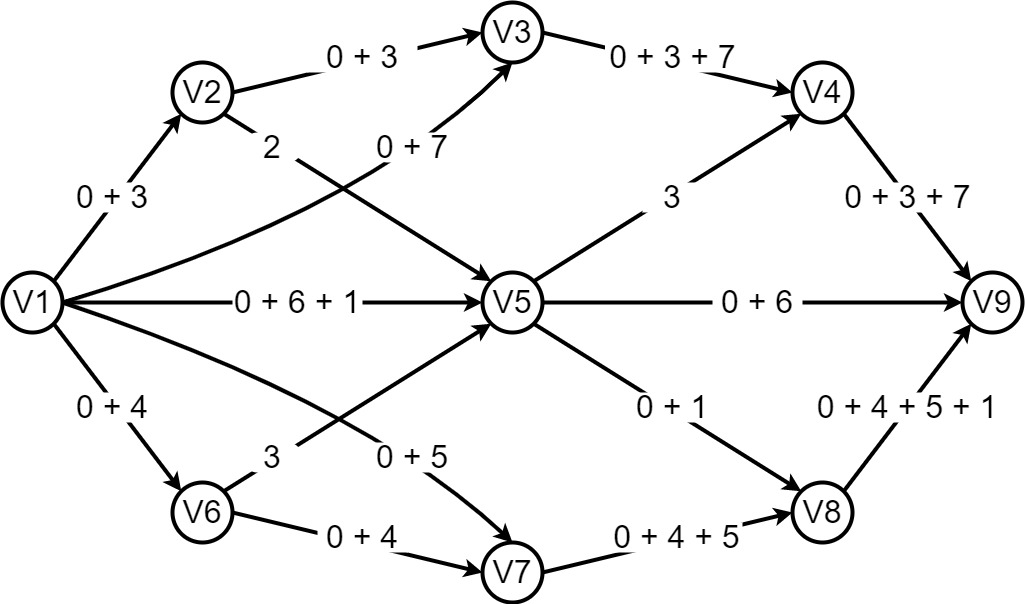
\includegraphics[width=\linewidth]{Images/graph14.jpg}
\caption{Построение полного потока}
\label{fig:image8}
\end{figure}
\noindent$v_1 \to v_2 \to v_3 \to v_4 \to v_9 \
\ min\{3,3,10,12 \}=3$ \\
$v_1 \to v_6 \to v_7 \to v_8 \to v_9 \
\ min\{4,4,9,12 \}=4$ \\
$v_1 \to v_5 \to v_9 \
\ min\{7,6 \}=6$ \\
$v_1 \to v_3 \to v_4 \to v_9 \
\ min\{11,10-3,12-3 \}=7$ \\
$v_1 \to v_7 \to v_8 \to v_9 \
\ min\{9,9-4,12-4 \}=5$ \\
$v_1 \to v_5 \to v_8 \to v_9 \
\ min\{7-6,2,12-9 \}=1$ \\
Величина полного потока $\Phi = 6 + 10 + 10 = 26$
\newpage
\subsection{Построение максимального потока}
\begin{figure}[!htb]
\centering
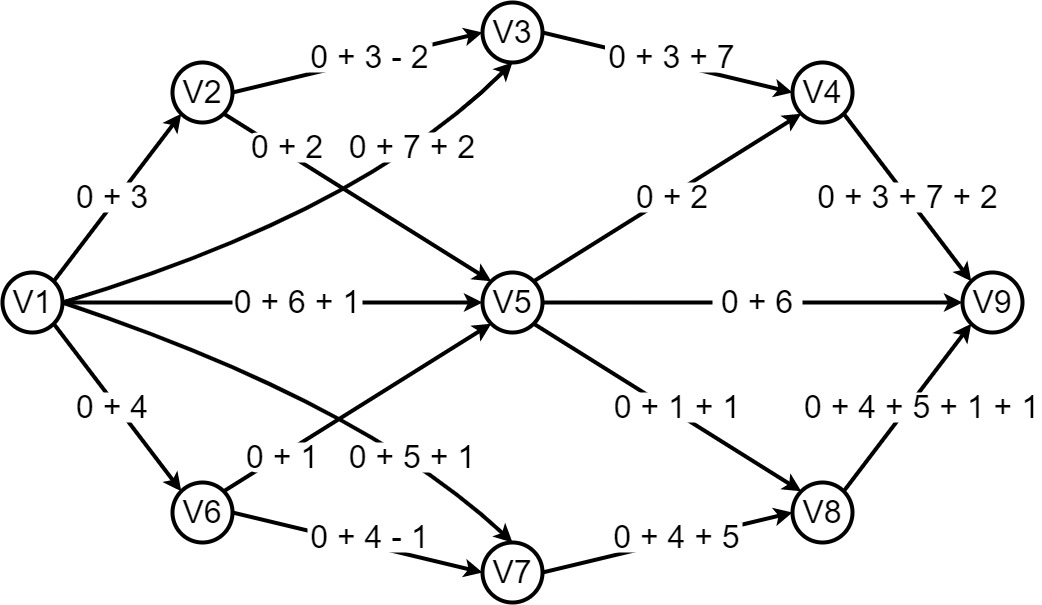
\includegraphics[width=\linewidth]{Images/graph15.jpg}
\caption{Построение Максимального потока}
\label{fig:image9}
\end{figure}
\newpage
\noindent$v_1 \to v_3 \to v_2 \to v_5 \to v_4
\to v_9 \ \ \Delta_1 =
min\{7,\underset{-}{3},2,3,10\}=2$ \\
$v_1 \to v_7 \to v_6 \to v_5 \to v_8
\to v_9 \ \ \Delta_2 =
min\{5,\underset{-}{4},3,1,10\}=1$ \\
Величина максимального потока $\Phi_{max} = 26 + 2 + 1 = 29$
\newpage
\section{Индивидуальное задание}
\subsection{Теоритические сведения. Описание работы алгоритма.}
\noindent\textbf{Определение 1.} Ориентированный граф $G = <V,X>$ - односторонне связанный, если для любой пары вершин $u_i, u_j (i \neq j)$ существует путь из $u_i$ в $u_j$ и из $u_j$ в $u_i$. \\
\textbf{Определение 2.} Матрица односторонней связности $T = \|t_{ij}\|$ орграфа - квадратная матрица порядка $n$ с элементами
\begin{center}
    $t_{ij} = \begin{cases}
    \text{1, если существует путь из $u_i$ в $u_j$}\\
    \text{0 в противном случае}
    \end{cases}$
\end{center}
\textbf{Определени 3.} Матрица сильной связности $\overset{-}{S} = \|\overset{-}{s_{ij}}\|$ орграфа - квадратная матрица порядка $n$ с элементами
\begin{center}
    $\overset{-}{s_{ij}} = \begin{cases}
    \text{1, если существует путь из $u_i$ в $u_j$ и из $u_j$ в $u_i$}\\
    \text{0 в противном случае}
    \end{cases}$
\end{center}
\textbf{Определение 4.} Сильно связной компонентой ориентированного графа $G = <V,X>$ называется такое максимальное множество вершин $C\subseteq V$, что для каждой пары вершин $u_i$ и $u_j$ из $C$ вершины $u_i$ и $u_j$ достижимы друг из друга.\\
\textbf{Определение 5.} Конденсацией орграфа $G$ называют такой орграф $G'$, вершинами которого служат компоненты сильной связности $G$, а дуга в $G'$ присутствует только если существует хотя бы одно ребро между вершинами, входящими в соответствующие компоненты связности.\\
\textbf{Определение 6.} Транспонированный граф для графа $G$ - ориентированного граф $G'$ с тем же набором вершин и с теми же дугами, но ориентация дуг этого графа противоположна ориентации дуг графа $G$
\newpage
\subsection{Алгоритм Косарайю}
Алгоритм предназначен для поиска компонент сильной связности в ориентированном графе и состоит из трёх шагов:
\begin{enumerate}
    \item [1)] Выполнить поиск в глубину (DFS), пока не будут «помечены» все вершины. Вершина считается «помеченной», когда ей присвоен индекс в порядке завершения рекурсивных шагов тактов DFS  (время выхода). Назовём одним тактом DFS поиск очередного дерева путей.
    \item [2)] Транспонировать исходный граф.
    \item [3)] Выполнить DFS в порядке убывания пометок вершин.
\end{enumerate}



Полученные деревья каждого такта DFS последнего шага являются компонентами сильной связности

Небольшое, но важное уточнение: время выхода следует считать следующим образом: изначально счётчик времени нулевой, а увеличивается он в двух случаях:

\begin{enumerate}
    \item [1)] Начало нового такта DFS
    \item [2)] Прохождение по ребру (при том, не важно, рекурсивный проход или нет)
\end{enumerate}
\newpage
\subsection{Логическая блок схема}
\begin{figure}[!htb]
\centering
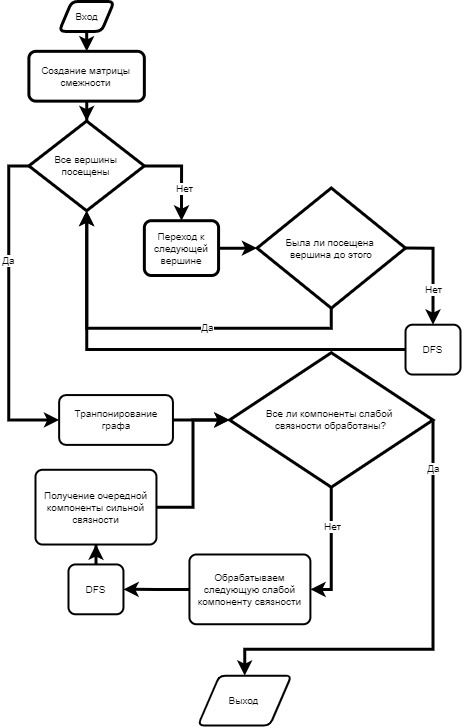
\includegraphics[scale = 0.9]{Images/graph16.jpg}
\caption{Блок схема}
\label{fig:image10}
\end{figure}

\newpage
\subsection{Оценка сложности алгоритма}
Сложность алгоритма алгоритма Косарайю составляет $O(n + m)$ где $n$ - количество вершин, $m$ - количество дуг.
\subsection{Тестовые примеры}
Для теста были взяты 2 примера из задания курсовой работы номер 1:
\begin{enumerate}
    \item[1)] Вариант 3\\$A = \begin{pmatrix}
0 & 1 & 1 & 0\\
0 & 0 & 1 & 1\\
1 & 0 & 0 & 0\\
1 & 1 & 1 & 0
\end{pmatrix}$
\item[2)] Вариант из методички\\$A =\begin{pmatrix}
0 & 1 & 1 & 0\\
0 & 0 & 1 & 1\\
0 & 0 & 0 & 0\\
1 & 1 & 1 & 0
\end{pmatrix}$
\end{enumerate}
Программа получила верные результаты
\begin{figure}[H]
\begin{minipage}[h]{0.47\linewidth}
\center{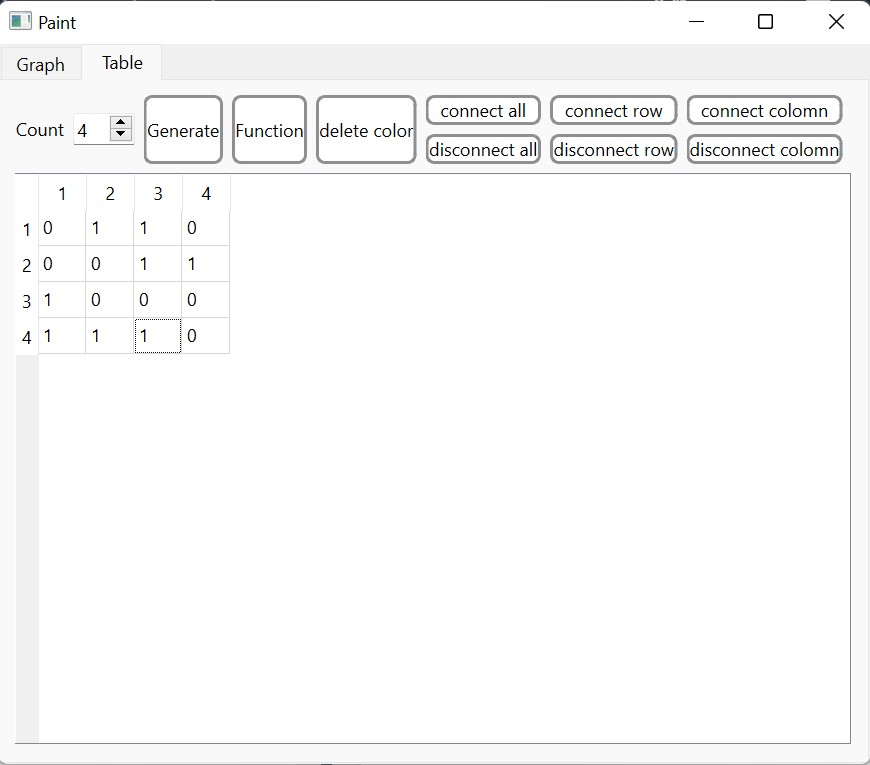
\includegraphics[width=1\linewidth]{Images/graph17.jpg}} 1) \\
\end{minipage}
\hfill
\begin{minipage}[h]{0.47\linewidth}
\center{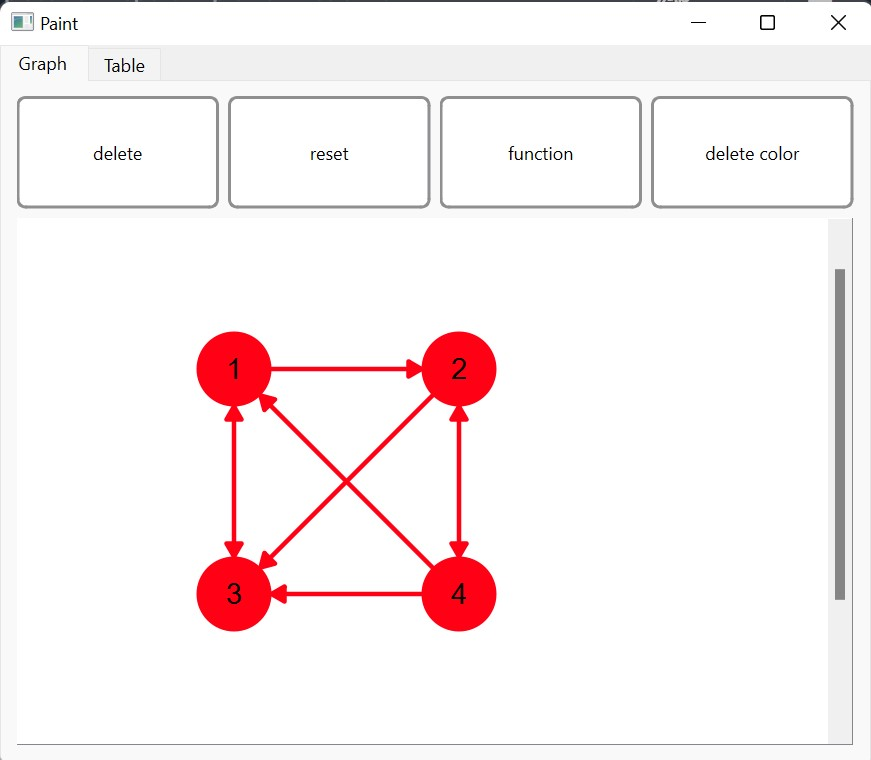
\includegraphics[width=1\linewidth]{Images/graph18.jpg}} \\2)
\end{minipage}
\vfill
\begin{minipage}[h]{0.47\linewidth}
\center{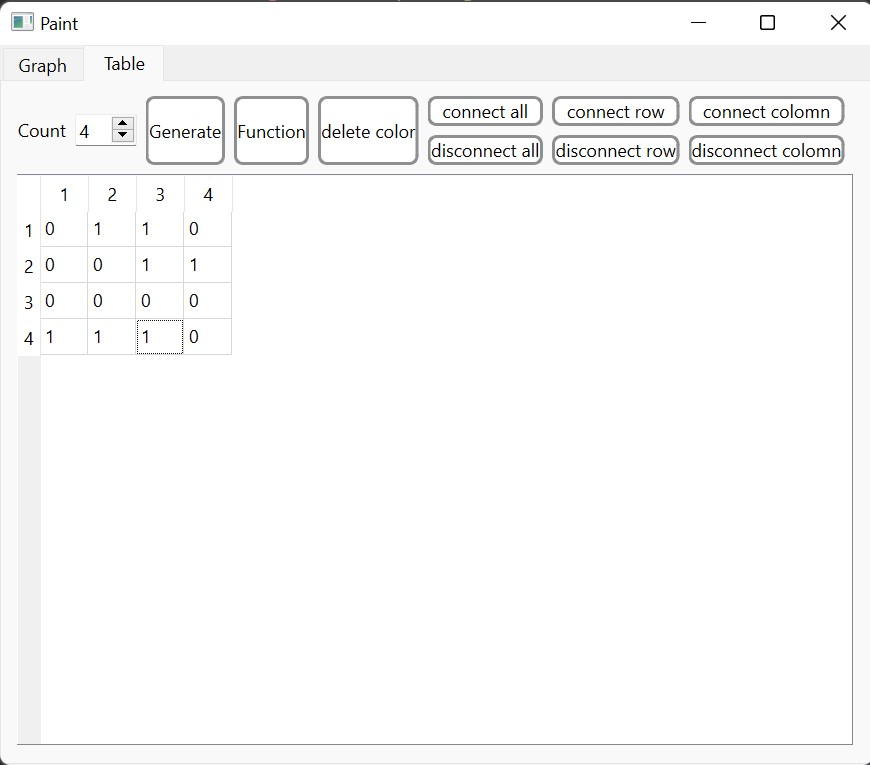
\includegraphics[width=1\linewidth]{Images/graph19.jpg}} 3) \\
\end{minipage}
\hfill
\begin{minipage}[h]{0.47\linewidth}
\center{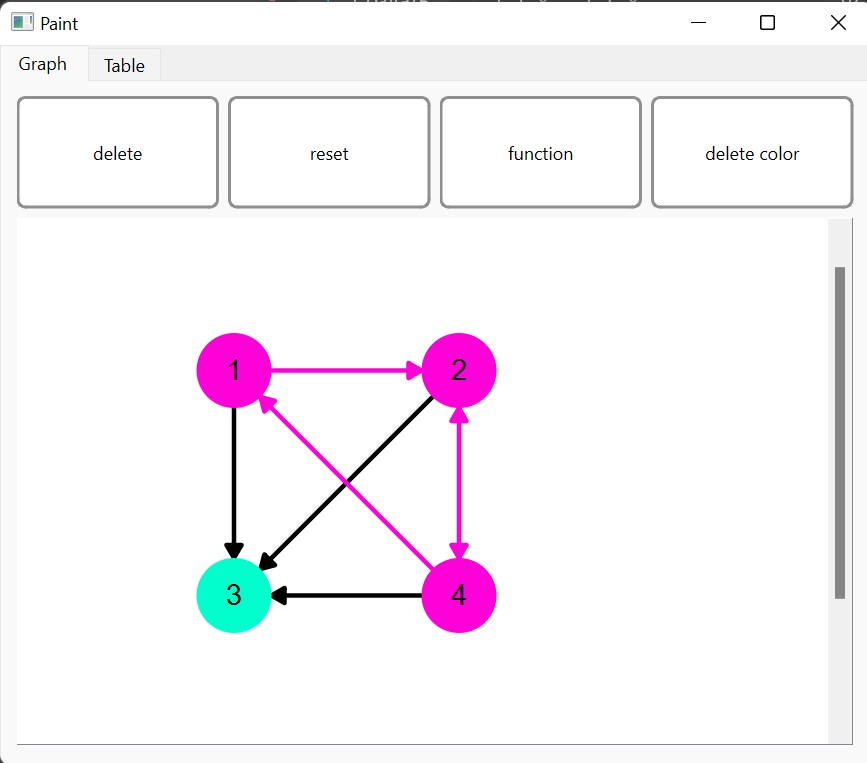
\includegraphics[width=1\linewidth]{Images/graph20.jpg}} 4) \\
\end{minipage}
\caption{Скриншоты программы}
\label{ris:experimentalcorrelationsignals}
\end{figure}
\newpage
\subsection{Пример прикладной задачи}
Нахождение загруженных узлов дорожной-транспортной сети, состоящей из $n$ транспортных узлов и $m$ магистралей




